% !TEX root=../index.tex

\chapter{Introduzione}
\label{cap:Introduzione}
\emph{Presentazione del problema, Stato dell'arte e descrizione delle caratteristiche peculiari del problema di riconoscimento.
Cenni sul funzionamento del sensore Kinect.
Head and Shoulder Profile.
Analisi del problema di classificazione.}

Il monitoraggio delle persone è un problema di visione artificiale di importanza fondamentale.
Sistemi di \emph{human sensing} vengono continuamente sviluppati ed utilizzati nei più disparati contesti applicativi. Sistemi di sorveglianza, apparecchiatura di supporto per missioni di salvataggio, dispositivi designati all'utilizzo in ambienti assistivi automatizzati e persino alcuni sistemi automatici per effettuare indagini di mercato utilizzano tecniche di percezione automatica delle persone dall'elaborazione dei dati acquisiti per mezzo di sensori.

Nel 2013 Zhu e Wong descrivono in \cite{Zhu13} un sistema allenabile di rilevamento e conteggio delle persone che attraversano una stanza.
Il riconoscimento della persona avviene elaborando i dati catturati dal sensore di profondità di un dispositivo Kinect, il quale è montato sul soffitto della stanza ed è puntato verso il pavimento. La crescente popolarità dei dispositivi Kinect, anche al di fuori degli ambienti videoludici, lo rende un interessante oggetto di studio.

\section{Head and Shoulder Profile}
\label{sec:hasp}
\begin{wrapfigure}{L}{0cm}
    \centering
    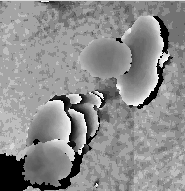
\includegraphics[width=5cm]{img/no_occlusion.png}
    \caption{Due persone in un ritaglio proveniente da un frame di profondità. Il frame è stato acquisito con il Kinect V1, a differenza di quello in figura \ref{fig:spatial_feature}, acquisito con il Kinect V2.}
    \label{fig:no_occlusion}
\end{wrapfigure}

In condizioni ottimali, la figura umana ripresa dall'alto è composta solamente dalla testa e dalle spalle.
Finchè si trova quasi in corrispondenza del sensore, nella parte centrale dell'immagine di profondità, la restante parte del corpo rimane quasi del tutto nascosta. Sulla posizione delle braccia non si possono fare delle assunzioni precise.

In figura \ref{fig:no_occlusion}, la figura dell'individuo a destra corrisponde a tale descrizione, mentre dell'altro è visibile parte del corpo ed una delle due spalle è nascosta dalla testa.
Nelle zone periferiche di un frame di profondità, l'immagine è soggetta alla \emph{distorsione prospettica} così come lo è quella di qualunque telecamere RGB.

Tale distorsione costituisce un disturbo, dal momento che la figura dello stesso soggetto varia a seconda della relativa posizione nell'area di visualizzazione.
Si vedrà più avanti come affrontare tale situazione, per il momento si considerano solamente le immagini proveniente dalle zone centrali dei frame (come quella in figura \ref{fig:spatial_feature}).

Un grande vantaggio dell'utilizzo del Kinect in questa configurazione è l'\emph{assenza di occlusione}.
Infatti, rispetto ai molteplici sistemi di riconoscimento frontali, i soggetti non possono nascondersi l'uno con l'altro al sensore.

Utilizzare le immagini di profondità significa ragionare con le distanze: piuttosto che cercare di descrivere l'immagine del profilo umano in termini di forma, deve essere descritto in termini di differenze di quota rispetto all'ambiente circostante.
Alla luce di ciò, si possono identificare i seguenti criteri descrittivi:

\begin{enumerate}
    \item L'immagine di una persona è caratterizzata da uno spazio vuoto di fronte ad essa e dietro di essa. Per \emph{spazio vuoto} si intende una regione la cui distanza dal sensore è circa quella del pavimento.
    \item A sinistra della spalla sinistra ed a destra della spalla destra del profilo dall'alto di una persona, sono presenti degli spazi vuoti.
    \item Tra la testa e le spalle vi è una differenza di altezza.

\end{enumerate}

\begin{wrapfigure}{R}{0cm}
    \centering
    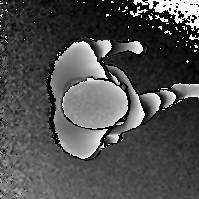
\includegraphics[width=4cm]{img/spatial_features.png}
    \caption{Una persona mentre cammina}
    \label{fig:spatial_feature}
\end{wrapfigure}

Di qui in avanti, con l'acronimo \emph{HASP} (\emph{Head And Shoulder Profile}), ci si riferirà proprio al profilo della persona ripreso dall'alto che soddisfa i criteri appena elencati.
